\section{Gaps in low mass discs (RL)}

%% We first describe results for weakly self-gravitating
%% discs $Q_0=8$ (giving $M_d=0.015M_*$) so that the gap remains 
%% gravitationally stable \citep{lin11b}. We also impose a dimensionless
%% kinematic viscosity $\hat{\nu}=2\times10^{-5}$ to suppress the Rossby
%% vortex instablity \citep{valborro07}. These parameter values
%% are typical for disc-planet simulations and yield stable/steady 
%% gap profiles. This will be useful reference cases to  
%% understand the unstable cases considered later.  

%% Fig. \ref{lvisc_steady_gap} shows the steady state gap profiles in terms of the relative
%% surface density and aspect-ratio at $t=200P_0$. Three levels of cooling are considered:
%% $\tbeta=0.1,\,1.0$ and $10.0$ (i.e. $t_c\Omega_k\simeq2.4,\,24$ and $240$). We refer to them as
%% fast, moderate and slow cooling cases, respectively. 

Long term simulation of vortices were done for $\tilde{\beta}=0.1,1.0$ and
 $\hat{\nu}=10^{-6},10^{-8},10^{-9}$ up to a total of 2000 orbits. Values
 of higher $\tilde{\beta}$ resulted generally in longer vortex lifetimes.
 The inviscid cases also were characterized by a sudden death of vortices
 while the higher viscosity case showed a gradual decrease in mode amplitudes
 attributed to the vortices.

Short term simulations of the linear phase of instability growth also distinguished
 the different effects of cooling rates. Simulations with higher
 $\tilde{\beta}$ were characterized by slower growth rates centered at the
 $m=2$ mode, lower density pertibations and vortex locations, and a more unitary aspect
 ratio for the vortices.

 \begin{figure}
   \includegraphics[scale=.42]{figures/stability_vis9betalow.ps}
   \caption{Mode intensity relative to $m=0$ for $\hat{\nu}=10^{-9}$ and $\tilde{\beta}=0.1$.}
 \label{stability_vis9lowb}
 \end{figure}

\begin{figure}
   \includegraphics[scale=.42]{figures/stability_vis9betamed.ps}
   \caption{Same as Fig. \ref{stability_vis9lowb} but $\hat{\nu}=10^{-9}$ and $\tilde{\beta}=1.0$. }
 \label{stability_vis9medb)}
 \end{figure}

\begin{figure}
   \includegraphics[scale=.42]{figures/stability_vis6betalow.ps}
   \caption{Same as Fig. \ref{stability_vis9lowb} but $\hat{\nu}=10^{-6}$ and $\tilde{\beta}=0.1$. }
 \label{stability_vis6lowb)}
 \end{figure}

\begin{figure}
   \includegraphics[scale=.42]{figures/stability_vis6betamed.ps}
   \caption{Same as Fig. \ref{stability_vis9lowb} but $\hat{\nu}=10^{-6}$ and $\tilde{\beta}=1.0$. }
 \label{stability_vis6medb)}
 \end{figure}
Same as \ref{stability_vis9lowb} but $\hat{\nu}=10^{-6}$ and $\tilde{\beta}=1.0$. 
\begin{figure}
   \includegraphics[scale=.60]{figures/analysis_sigma50lowb.ps}
   \caption{Density pertibation of disk at time=$50t_p$ with $\hat{\nu}=10^{-9}$ and $\tilde{\beta}=0.1$. }
 \label{shortterm_lowb)}
 \end{figure}

\begin{figure}
   \includegraphics[scale=.60]{figures/analysis_sigma50highb.ps}
   \caption{Density pertibation of disk at time=$50t_p$ with $\hat{\nu}=10^{-9}$ and $\tilde{\beta}=10.0$. }
 \label{shortterm_highb)}
 \end{figure}

%we checked that open bc doesn't affect gap structure
%checked that t=200 plots are similar to t=100 

%surface density plot

%aspect-ratio plot

%general vortensity plot 



%% \begin{figure}
%%   \includegraphics[scale=.42,clip=true,trim=0cm 1.8cm 0cm 0cm]{figures/compare_profiles_dens020.ps}\\
%%   \includegraphics[scale=.42]{figures/compare_profiles_h020.ps}
%%   \caption{Steady-state gap profiles in a low mass viscous disc. The
%%     surface density perturbation (top) and disc aspect-ratio (bottom)
%%     are shown as a function of the cooling parameter:  
%%     $\tbeta=0.1$ (solid, fast cooling), $\tbeta=1$ (dotted,
%%     moderate cooling) and $\tbeta=10$ (dashed, slow
%%     cooling). \label{lvisc_steady_gap}}  
%% \end{figure}



%% \begin{figure}
%%   \includegraphics[scale=.42]{figures/compare_profiles_gvort020.ps}
%%   \caption{Gap structure in a low mass viscous disc, in terms of the
%%     perturbed generalized vortensity as a function of the cooling
%%     parameter. \label{lvisc_steady_gvort}} 
%% \end{figure}






\section{Gaps in massive discs (MKL)}
%% We first examine disc models with $Q_o=1.5$. We set the physical
%% viscosity $\hat{\nu}=10^{-9}$, so that the only energy source is
%% through shock-heating (via artificial viscosity) and the $\mathcal{C}$
%% function when $e\Sigma<e_i\Sigma_i$. The numerical resolution is
%% $N_r\times N_\phi = 512\times 1024$.   

%% %Since we are primarily concerened with gap stability, it is important
%% %to first examine the gap structured opened by the planet as a function
%% %of cooling. 
%% Fig. \ref{gvort1d_q1d5} compares the gap structure in terms of the GV profile for three
%% levels of cooling: $\tilde{\beta}=0.1$, $\tilde{\beta}=1$ and
%% $\tbeta=10$. For convenience we will refer to these cases as fast,
%% intermediate and slow cooling, respectively. The snapshot is taken at
%% $t=30P_0$, just after the planet is fully introduced. 

%% In terms of the GV profile, the qualitative features of the planetary
%% gap --- localized GV extrema at the gap edges --- remain unchanged
%% despite two orders of magnitude difference in the cooling rate.   


%% \begin{figure}
%% %  \includegraphics[scale=.42,clip=true,trim=0cm 1.8cm 0cm 0cm]{figures/dens1d_q1d5_003_global.ps}\\
%% %  \includegraphics[scale=.42]{figures/gvort1d_q1d5_003_global.ps}
%%   \caption{Gap structure in terms of the perturbed surface density
%%     (top) and perturbed generalized
%%     vortensity (bottom), as a function of the cooling parameter:  
%%     $\tbeta=0.1$ (solid, fast cooling), $\tbeta=1$ (dotted,
%%     intermediate cooling) and $\tbeta=10$ (dashed, slow
%%     cooling). \label{gvort1d_q1d5}} 
%% \end{figure}

%% \begin{figure*}
%% %  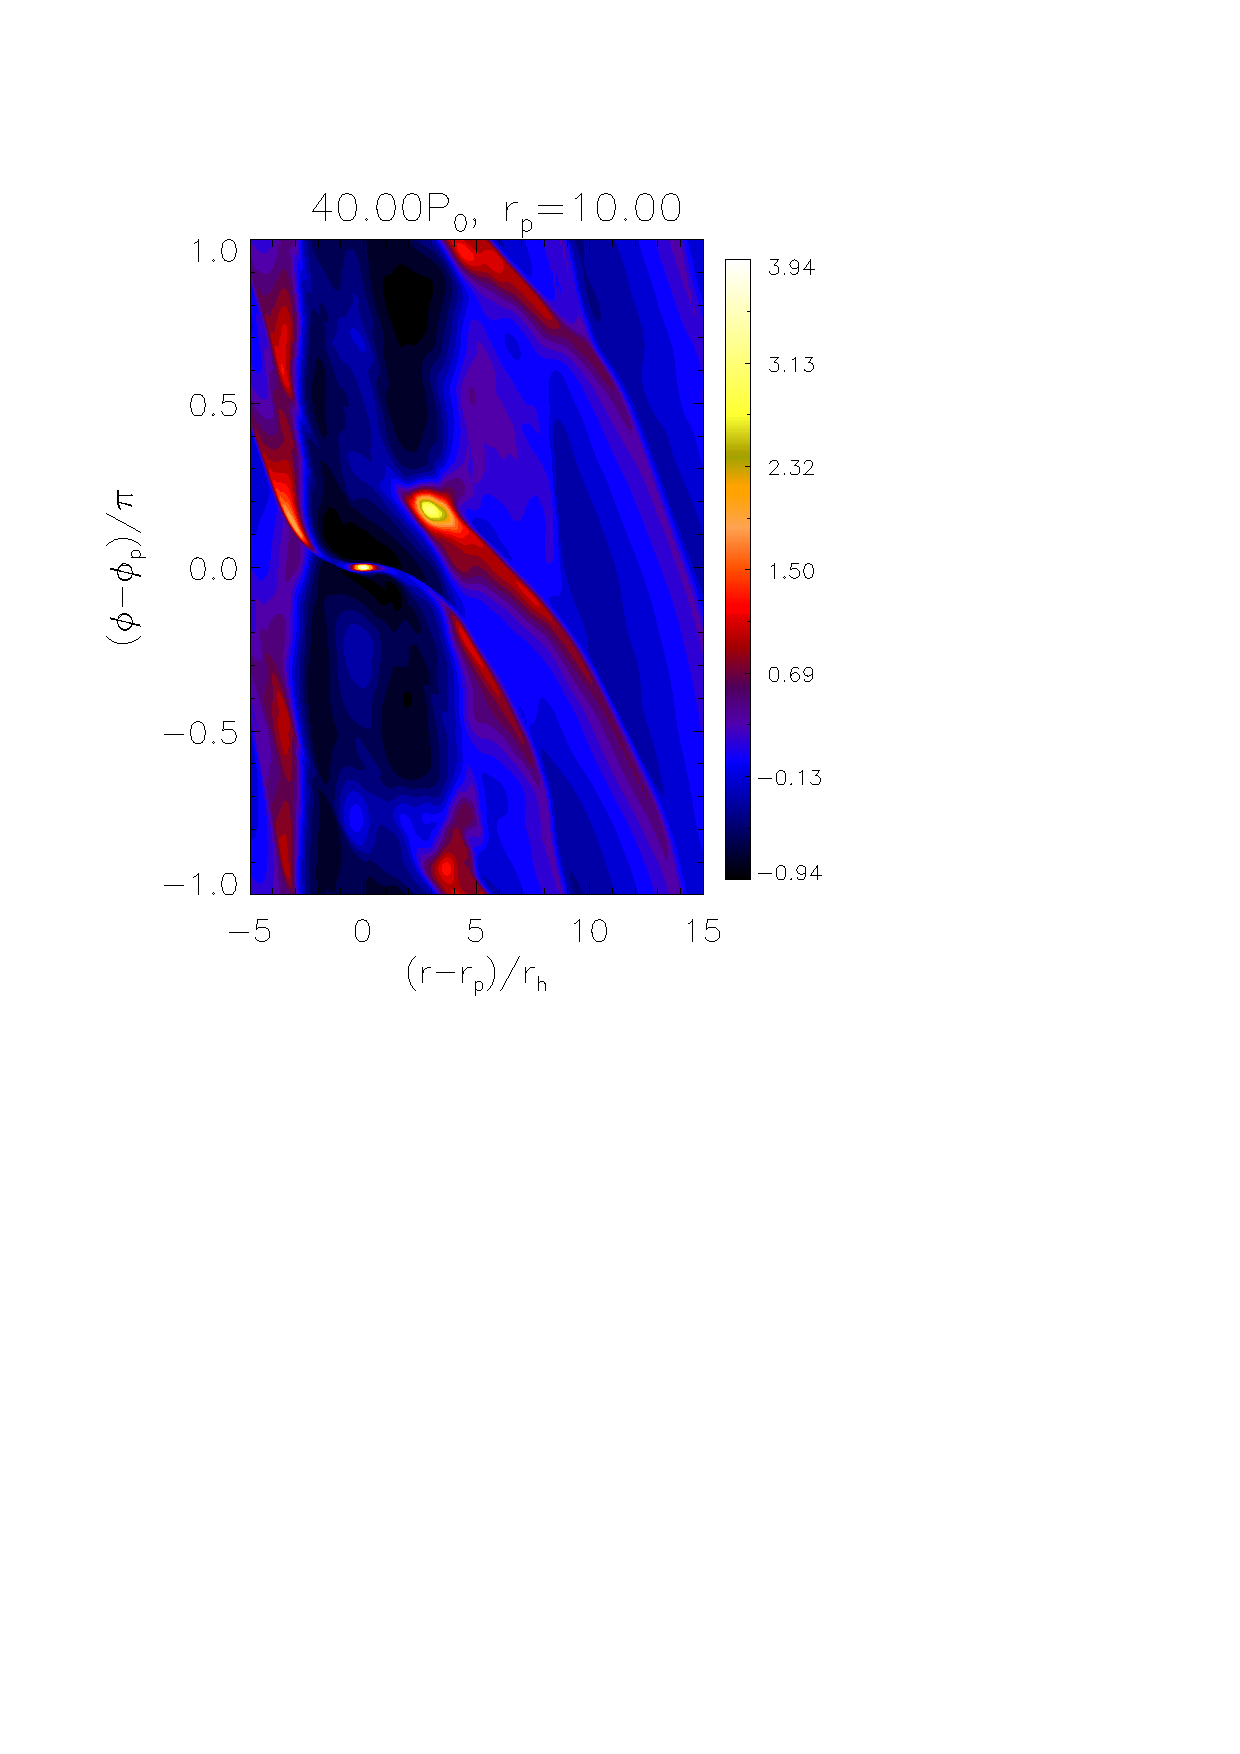
\includegraphics[scale=.55,clip=true,trim=0cm 0cm 0cm
%% %    0cm]{figures/noniso0_HR_dens004}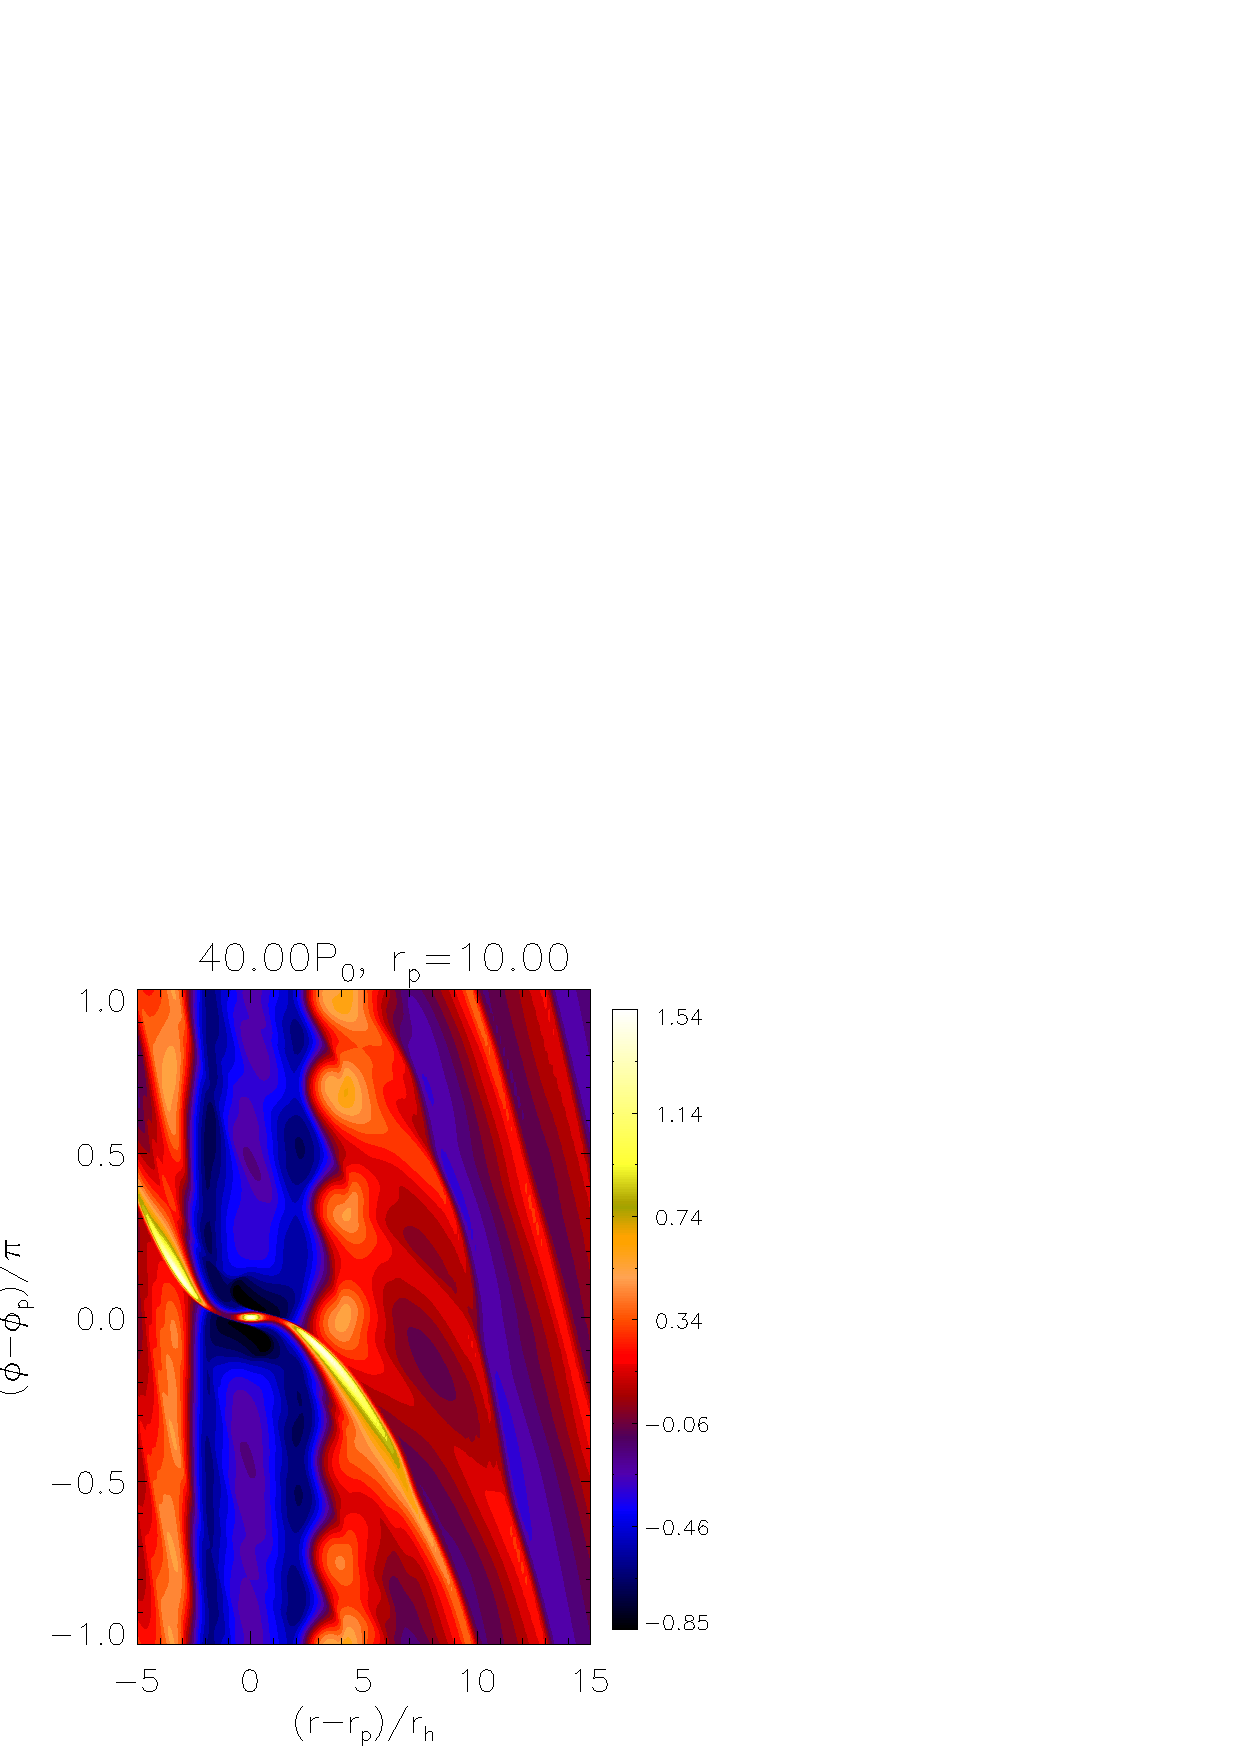
\includegraphics[scale=.55,clip=true,trim=2.26cm 0cm 0cm
%% %    0cm]{figures/noniso1_HR_dens004}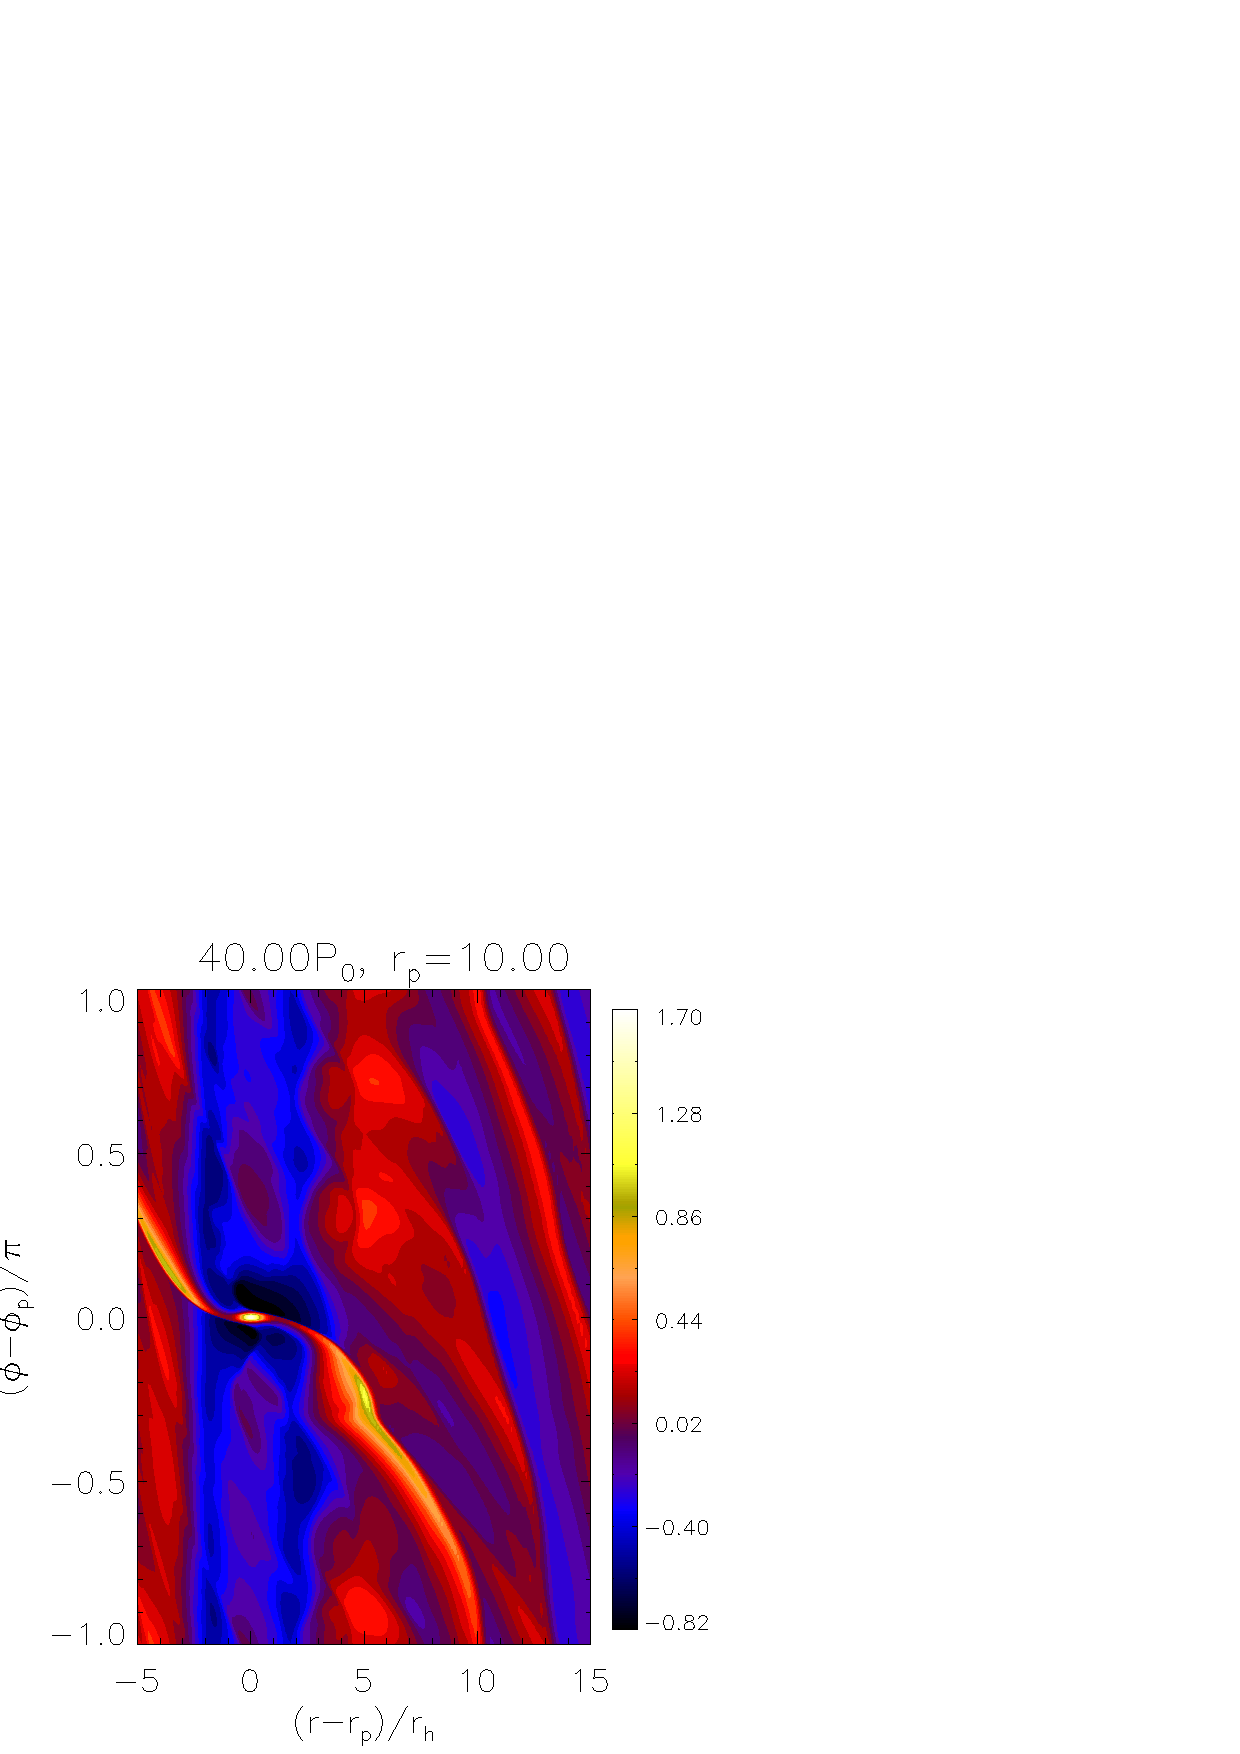
\includegraphics[scale=.55,clip=true,trim=2.26cm 0cm 0cm
%% %    0cm]{figures/noniso2_HR_dens004}
%%   \caption{Gap instability in the heavy disc model, as a function of
%%     the cooling parameter: $\tbeta=0.1$ (left), $\tbeta=1$ (middle)
%%     and $\tbeta=10$ (right). The relative surface density
%%     perturbation is shown. \label{polarxy_q1d5}} 
%% \end{figure*}
